\chapter{Supporting Information for the Example Manuscript}\label{app:example-si}

Appendices are included after the \verb|\appendix| declaration in the main file.
Figures and tables in appendices should be numbered with appendix letters, such
as Figure~\ref{fig:appendix-example} and Table~\ref{tab:appendix-example}.

\section{Supplemental Figure}

\begin{figure}[htbp]
  \centering
  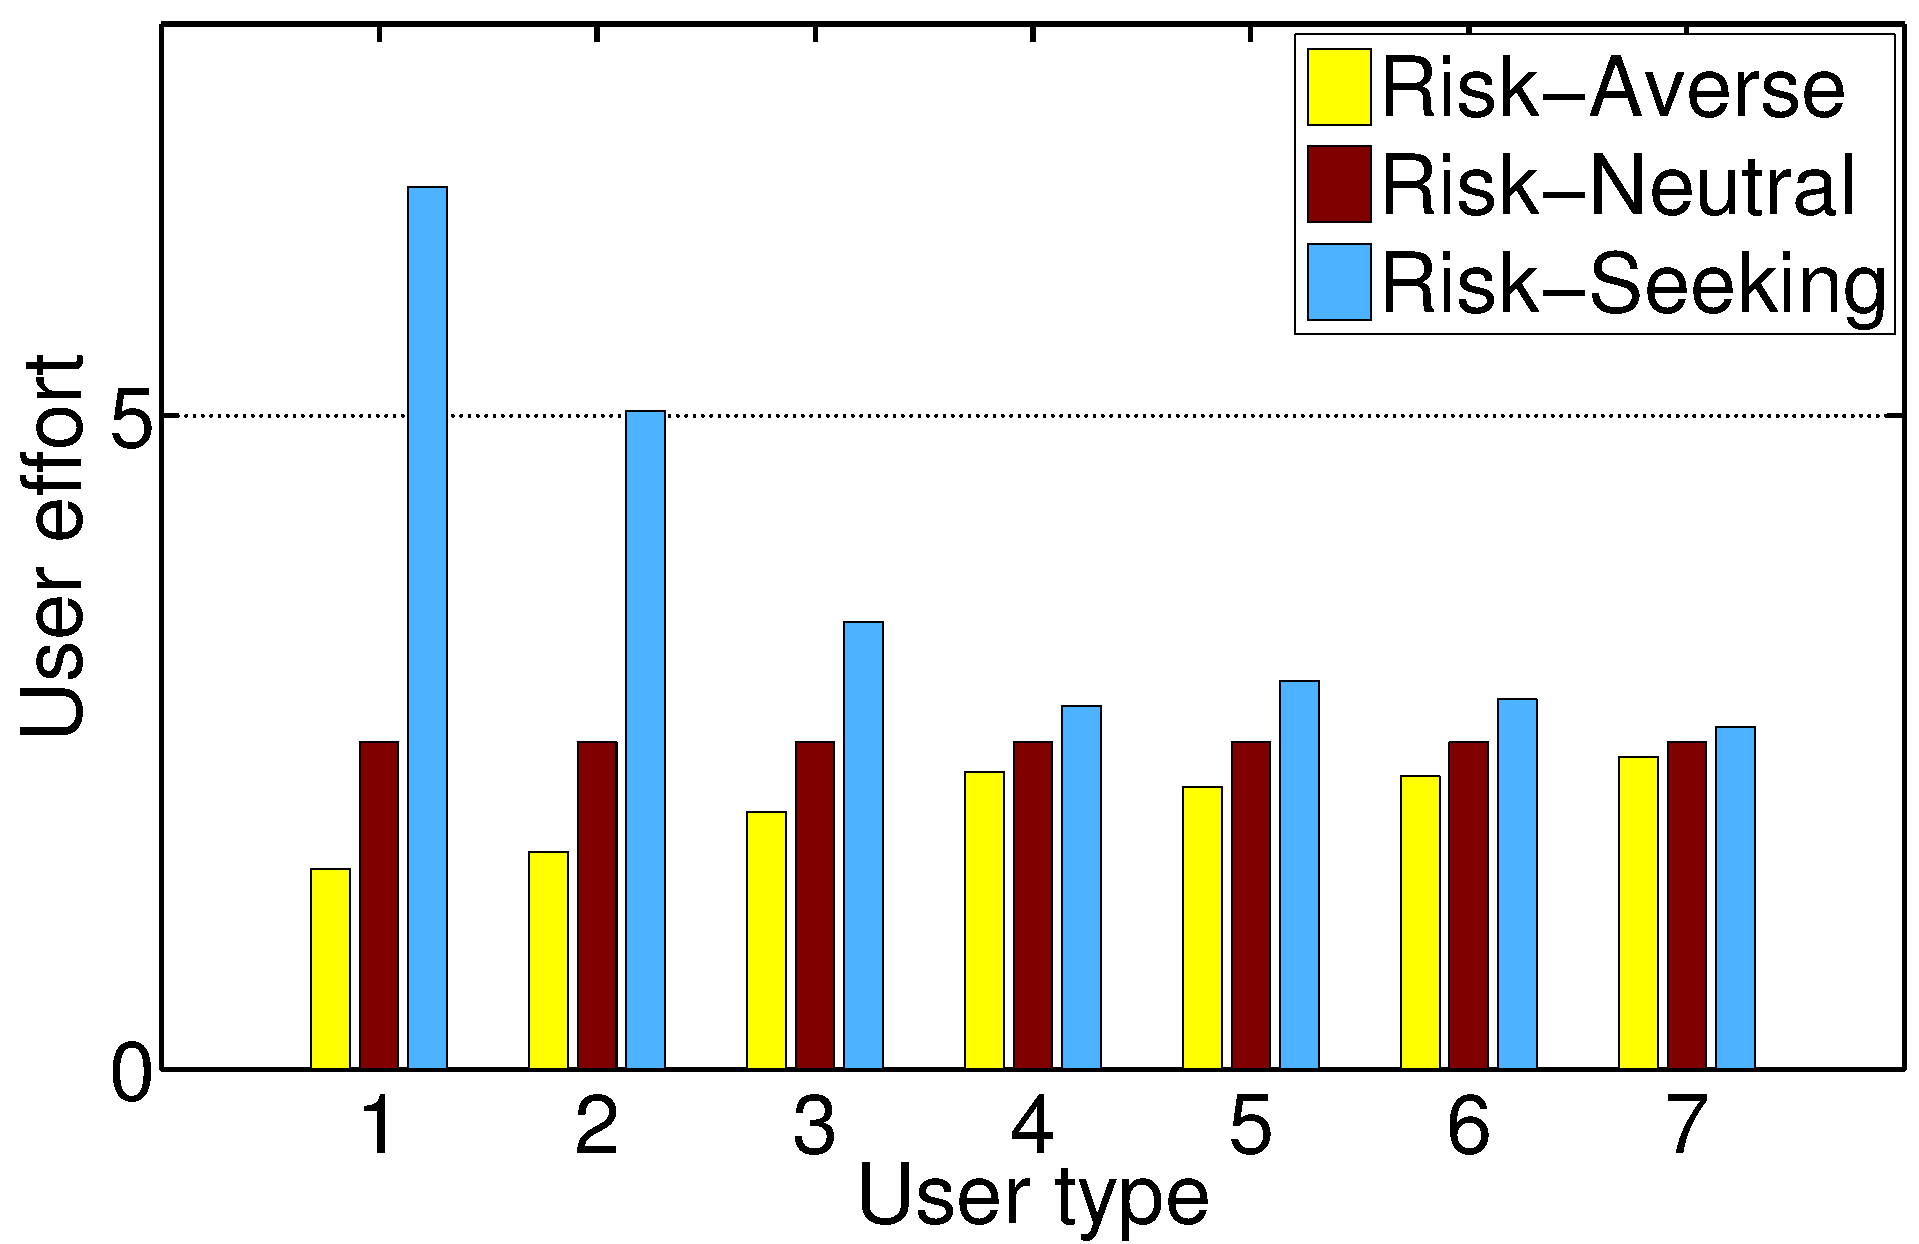
\includegraphics[width=0.75\linewidth]{fig4}
  \caption{Example appendix figure. In the compiled document, this should appear
  as Figure A.1 and should be listed in the List of Figures.}
  \label{fig:appendix-example}
\end{figure}

\section{Supplemental Table}

\begin{table}[htbp]
  \caption{Example appendix table. In the compiled document, this should appear
  as Table A.1 and should be listed in the List of Tables.}
  \label{tab:appendix-example}
  \centering
  \begin{tabular}{ll}
    \toprule
    Item & Notes \\
    \midrule
    Figure numbering & Uses appendix letter and figure number \\
    Table numbering & Uses appendix letter and table number \\
    Cross-references & Use \verb|\ref| or related LaTeX commands \\
    \bottomrule
  \end{tabular}
\end{table}
